\chapter{Marco teórico}

	Para realizar la estimación de la mirada de las personas en un plano virtual enfrente de ellas es necesario conocer algunos conceptos, definiciones y algunos conocimientos que sirvan de apoyo al desarrollo del presente trabajo de tesis. En este capítulo se describen las bases para llevar a cabo el proyecto, dichas bases consisten principalmente de visión computacional, geometría proyectiva, algoritmos de aprendizaje supervisado, algoritmos de optimización numérica....

   %Añadir un parrafo de lo que aporta el de nosotros (plano)
   %Tomando en cuenta las consideraciones anteriores 
   %El proyecto de tesis propuesto además de estimar la pose de la cabeza mediante algoritmos de aprendizaje automático utilizará dichos algoritmos para asociarle a las cabezas humanas una región 

   
   \section{Detector de rostros de Viola y Jones}
  Como ya se ha mencionado anteriormente para estimar la mirada con precisión se necesita un sistema de detección y seguimiento de ojos además de múltiples cámaras y el sistema de estimación de pose de la cabeza, habiendo señalado lo anterior cabe destacar que el proyecto que se desarrollará más que estimar la mirada con precisión (además de la pose de la cabeza) representándola como un vector normal al iris,  se pretende estimar una región en un plano virtual enfrente de ellas, la región indicaría lo que están observando las personas de la escena que tienen enfrente. \\
   
   En el presente proyecto para la estimación de la pose de la cabeza de las personas en primer lugar se debe detectar dónde se encuentran los rostros (como se ha mencionado) para luego estimar su pose, ya que el sistema consiste de muchas etapas, se requiere que la detección se haga lo más rápido posible y eficientemente,  por lo tanto se decidió utilizar uno de los algoritmos de detección más utilizados y rápidos que existen: el clasificador basado en características tipo Haar en cascada. Este método fue propuesto por Paul Viola y Michael Jones en 2001 en el artículo Rapid Object Detection using a Boosted Cascade of Simple Features, el método consta principalmente de las siguientes etapas.
   
   \subsection{Imagen integral}
   En esta etapa se utiliza una representación intermedia de la imagen conocida como imagen integral o también conocida como tablas de áreas sumadas [Crow 1984]. En la imagen integral a cada pixel de la imagen se le asocia un valor representando la suma de los valores de los píxeles que se encuentran arriba y a la izquierda de él, así como también se le suma su valor de píxel. Este tipo de representación tiene como principal ventaja la rápida estimación del valor de los píxeles de subregiones de la imagen.
   \begin{figure}[htbp]
   	\centering
   	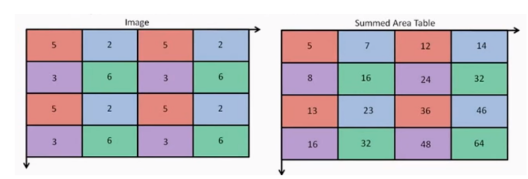
\includegraphics[width=0.7\textwidth]{./pictures/imagenIntegral}
   	\caption{Ejemplo de imagen integral}\label{fig: figura}
   \end{figure}
   El detector de Viola y Jones clasifica las imágenes basado en el valor de simples características, los sistemas basados en características operan muchos más rápido que los basados en píxeles. La imagen integral puede ser usada para estimar el valor de características tipo Haar, las características Haar se visualizan como rectángulos adyacentes blancos y negros, el valor que generan se calcula de la diferencia de la suma de los pixeles en el área blanca menos la suma de los del área negra, la adyacencia que presentan los rectángulos permite reutilizar algunos valores. El conjunto de características rectangulares ofrece una muy buena representación de imágenes la cual soporta un efectivo entrenamiento.
   
   \begin{figure}[htbp]
   	\centering
   	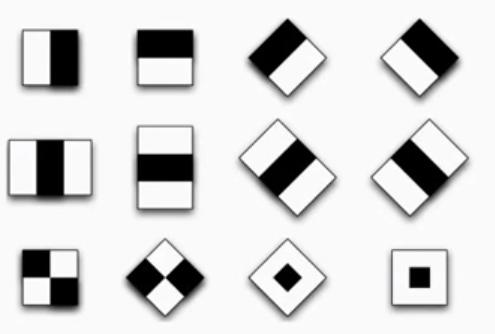
\includegraphics[width=0.4\textwidth]{./pictures/haar}
   	\caption{Características Haar}\label{fig: figura}
   \end{figure}
   
   \subsection{Algoritmo AdaBoost}
   Los métodos de Boosting [Friedman et al 2000] básicamente consisten en combinar la eficiencia de muchos clasificadores débiles para producir un poderoso consejo o comité clasificador. El algoritmo Adaboost es el método más usado y práctico de los algoritmos de Boosting. La idea general del AdaBoost consiste en que los ejemplos que son clasificados erróneamente obtienen mayor peso en las iteraciones siguientes, esto significa que los ejemplos que se encuentran cerca de la frontera de decisión son generalmente más difíciles de clasificar y por lo tanto se les asigna mayores pesos después de unas cuantas iteraciones. La idea de reasignación de pesos en el conjunto de entrenamiento es esencial en los métodos de Boosting.
   El detector de Viola y Jones se entrenó con conjuntos de imágenes etiquetadas como positivas y negativas, el algoritmo de AdaBoost fue utilizado para entrenar al clasificador y seleccionar un conjunto pequeño con las características Haar más importantes de una muy amplia biblioteca de posibles características. Como resultado final del proceso de entrenamiento el algoritmo de AdaBoost produce un clasificador robusto que tiene la forma de un perceptrón, una combinación de clasificadores débiles en el que cada clasificador tiene asociado una sola característica Haar y un umbral. Resumiendo lo anteriormente mencionado, la utilización del algoritmo de clasificación AdaBoost permite encontrar las características que mejor separan los ejemplos positivos de los negativos. Una de las ventajas clave por la cual fue elegido AdaBoost como algoritmo seleccionador de características por Viola y jones en su detector, es la increíble velocidad que presenta; usando AdaBoost, un clasificador de 200 características puede ser construido en alrededor 10-11 operaciones de procesador. Las primeras características seleccionadas por AdaBoost tienen mucho sentido y son fáciles de interpretar, una de esas característica parece enfocarse en la propiedad de que la región de los ojos es por lo regular más oscura que la región de la nariz y las mejillas.
   \begin{figure}[htbp]
   	\centering
   	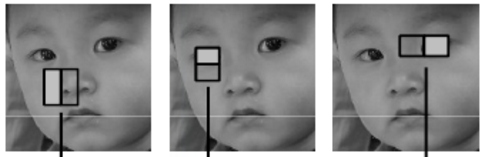
\includegraphics[width=0.7\textwidth]{./pictures/adaboost}
   	\caption{Características tipo Haar sobrepuestas}\label{fig: figura}
   \end{figure}
   
   \subsection{Filtro con estructura en cascada.}
   El último componente importante del Detector de Viola y Jones es la estructura en cascada que se forma con la combinación de unos cuantos clasificadores mejorados (boosted), estos clasificadores son usados para rechazar la mayor??a de las subregiones negativas (sin rostros de personas) y poner atención en regiones de la imagen más prometedoras, es decir, las regiones que presenten el rostro de alguna persona. Este método es muy eficiente ya que la mayor??a de las sub-ventanas o subregiones son rechazadas en etapas tempranas. Se le denominó estructura en ?cascada? debido a la forma que presenta al momento de procesar las sub- ventanas. Las sub-ventanas de la entrada del detector pasan a través de una serie de nodos, cada nodo toma una decisión binaria y dependiendo de la decisión la subregión se mueve al siguiente nodo o se rechaza. El número de clasificadores débiles presentes en cada nodo incrementa conforme la sub-ventana se va moviendo a los siguientes nodos, por ejemplo, en el primer nodo contiene un clasificador débil, el segundo 10, el tercero 25, el cuarto 50 y as?? sucesivamente. Teniendo pocos clasificadores en etapas tempranas es otra forma de mejorar la velocidad del detector y esto de alguna forma compensa el costo de evaluar cada caracter??stica Haar en diferentes escalas y posiciones de la imagen.
   \begin{figure}[htbp]
   	\centering
   	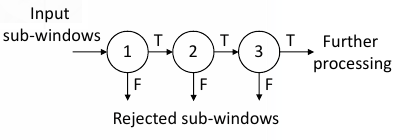
\includegraphics[width=0.7\textwidth]{./pictures/cascada}
   	\caption{Diagrama de nodos}\label{fig: figura}
   \end{figure}
   
   El detector de rostros descrito en esta sección tiene incontables aplicaciones y debido la velocidad de la detección puede ser utilizado en aplicaciones que requieran detección en tiempo real. Uno de los aspectos más interesantes del método de Viola y Jones es que no se limita a la detección de rostros, puede ser modificado para sistemas detectores de otro tipo de patrones en las imágenes, por ejemplo automóviles, peatones y recientemente utilizado para la detección de la enfermedad de Chagas, mediante las muestras de sangre de los infectados [Uc Cetina et al 2015].
   \begin{figure}[htbp]
   	\centering
   	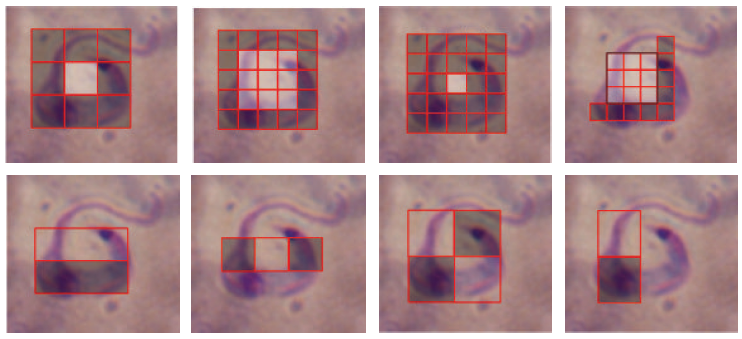
\includegraphics[width=0.7\textwidth]{./pictures/chagas}
   	\caption{Detección de chagas en la sangre mediante el método de Viola y Jones}\label{fig: figura}
   \end{figure}
   
   \section{Matrices de Rotación}
   \section{Homografía}
   \section{Modelo pinhole de cámara}
   \section{Calibración de cámaras y corrección de imágenes}
   \section{Optimización numérica y Levenberg-Marquardt}
   \section{Aprendizaje Automático}
   \section{Redes neuronales artificiales}
   \section{Descriptores HOG}

   Se comenzará esta sección describiendo de manera general qué es un descriptor de características ``feature descriptor'' y luego se hará mención en específico de los descriptores tipo HOUGH. Una descriptor de características de una imagen o de una región de una imagen es que simplifica la imagen extrayendo información útil y desechando toda la información extraña.
   Tipicamente un descriptor convierte una imagen de tamaño igual a $ancho$ x $largo$ x $3$ (canales) a un vector de características de longitud $n$, en el artículo original [Dalal et al, 2005] se utiliza como ejemplo una imagen de tamaño 64 x 128 x 3 por lo que la longitud del vector $n$ es de 3780. A partir de ahora se utilizará como ejemplo las mismas dimensiones que las utilizadas en el artículo original, sin embargo, hay que tener en cuenta que se puede utilizar HOG para cualquier dimensión en las imágenes.\\
   %%Qué tipos de características son "útiles para nuestro proyecto"
   La siguiente pregunta que sale a la vista es ¿qué tipo de características son útiles para la etapa de clasificación del presente trabajo de tesis?. Al utilizar el descriptor de características se busca que cumpla los siguientes requisitos:
   \begin{itemize}
		\item Ayudar a que las imágenes con rostros (pueden ser de diferentes personas) que miran la misma región en pantalla sean agrupados en el mismo conjunto
		\item Ayudar a que las imágenes con rostros que miran diferentes regiones en pantalla sean agrupados en conjuntos diferentes
   \end{itemize}
En los descriptores HOG, la distribución (histograma) de las direcciones de los gradientes (gradientes orientados) son usados como características. Los gradientes (derivadas en $x$ y $y$) de una imagen son útiles porque la magnitud de los gradientes es mayor alrededor de los bordes y las esquinas (regiones con cambios abruptos de intensidad) y es bien conocido que los bordes y las esquinas ofrecen mucha más información sobre la forma del objeto que las regiones planas.

\subsection{Cálculo del histograma de gradientes orientados}
A continuación se describirá como se realiza el cálculo del descriptor HOG tomando como ejemplo una región de la imagen \ref{fig: hogExample} para detectar peatones, como en el artículo original.

  \begin{figure}[htbp]
     	\centering
     	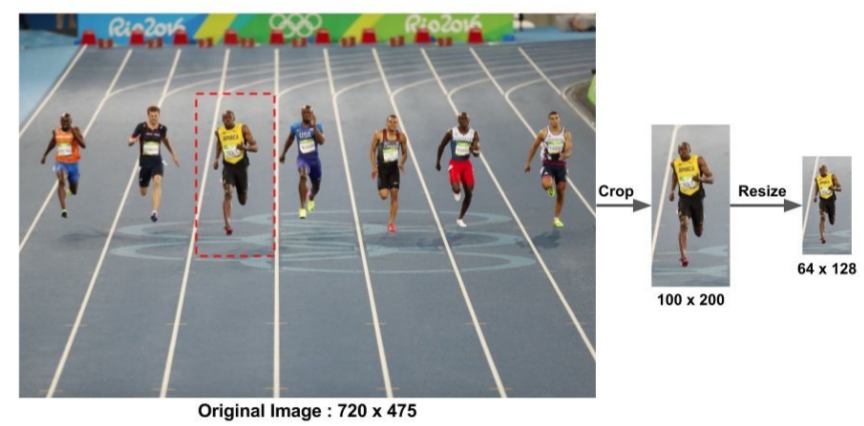
\includegraphics[width=0.5\textwidth]{./pictures/hogExample}
     	\caption{Imagen de ejemplo para HOG}\label{fig: hogExample}
  \end{figure}
  
 \subsubsection{Paso 1: Preprocesamiento y normalización}
 El descriptor HOG es calculado en una región de la imagen de 64x128, generalmente dichas regiones son analizadas a multiples escalas y en muchas locaciones, la única restricción es que las regiones siendo analizadas tengan una proporción fija. En este caso, las regiones necesitan tener una proporción de 1:2. Por ejemplo, ellas pueden ser 100x200, 128x256 pero no 101x205.\\
 En la figura \ref{fig: hogExample} se puede observar que se eligión una imagen de 720x475 y en ella se seleccionón una región de 100x200 para calcular el descriptor HOG, esta región se redimensionó a 64x128.

 \subsubsection{Paso 2: Calcular los gradientes de la imagen}
 Para calcular el descriptor HOG es necesario calcular primero los gradientes horizontales y verticales, esto se logra facilmente filtrando la imagen con los siguientes kernels:
  \begin{figure}[htbp]
  	\centering
  	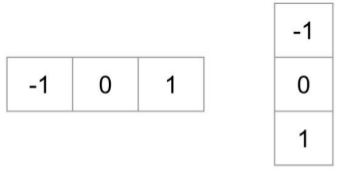
\includegraphics[width=0.3\textwidth]{./pictures/hogFilter}
  	\caption{Kernels}\label{fig: hogFilter}
  \end{figure} 
  
  La magnitud y dirección del gradiente se obtienen aplicando las siguientes fórmulas:
  	\begin{eqnarray}
	  	g-\sqrt{g^2_x+g^2_y} \\
	  	\theta-arctan\frac{g_y}{g_x}
  	\end{eqnarray}
 En la figura \ref{fig: hogFilter} se observan los resultados de los gradientes:
  \begin{figure}[htbp]
  	\centering
  	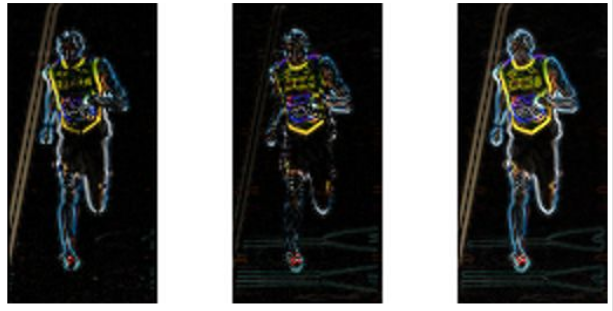
\includegraphics[width=0.5\textwidth]{./pictures/hogGradients}
  	\caption{Izquierda:  valor absoluto del gradiente x. Centro: valor absoluto del gradiente y. Derecha: magnitud del gradiente}\label{fig: hogFilter}
  \end{figure}  
  Nótese que la magnitud del gradiente se intensifica donde sea que haya cambios bruscos de intensidad y ninguno de los gradientes anteriores se intensifica en las regiones suaves de la imagen.\\
  Los gradientes de la imagen remueven bastante información no esencial y destaca los contornos, por ejemplo, en la imagen de los gradientes \ref{fig: hogFilter} se pudiera deducir facilmente que es una persona corriendo.\\
  En HOG, en cada pixel, el gradiente tiene una magnitud y una dirección. La magnitud del gradiente de un pixel es el máximo de la magnitud de los gradientes los tres canales (en imágenes RGB), y el ángulo es el ángulo correspondiente al máximo gradiente.
   
   \subsubsection{Paso 3: Cálculo del Histograma de gradientes}
   En este paso la región seleccionada es dividida en celdas de 8x8 y un histograma de gradientes es calculado para cada celda de 8x8. El criterio para la selección de la dimensión de las celdas (8x8), se realiza en base a la dimension del objeto en la imagen que se quiere analizar, tomando el ejemplo del corredor (cuya dimensión es de 64x128), las celdas de 8x8 son lo suficientemente grandes para capturar características interesantes (el rostro, la parte superior de la cabeza, etc.)
   
     \begin{figure}[htbp]
     	\centering
     	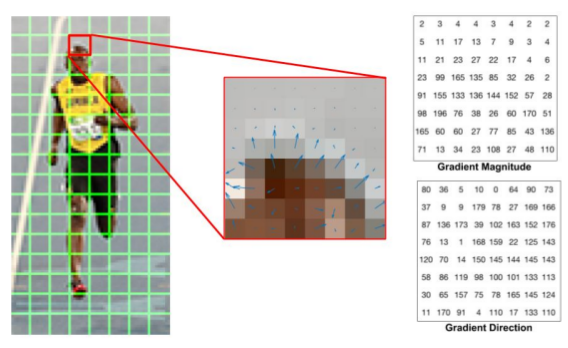
\includegraphics[width=0.5\textwidth]{./pictures/hog8x8}
     	\caption{Valores de los gradientes de celda 8x8}\label{fig: hog8x8}
     \end{figure}
     En la figura \ref{fig: hog8x8} se presenta una celda del objeto analizado con los valores de sus gradientes, en el cuadro del centro se pueden apreciar los pixeles en una celda con flechas sobrepuestas mostrando la dirección y magnitud de los gradientes. Nótese como la dirección de la flecha apunta hacia la dirección del cambio de intensidad y la magnitud muestra que tan grande es la diferencia.\\
     A continuación se crea el histograma de gradientes de las celdas de 8x8, el histograma contiene 9 bins correspondientes a los ángulos 0, 20, 40...160. En \ref{fig: hogCalc} se encuentra el proceso del cálculo del histograma, la selección del bin (celda del arreglo) está basado en la dirección y el valor que va dentro del bin es la magnitud del gradiente.
     
\begin{figure}[htbp]
   	\centering
   	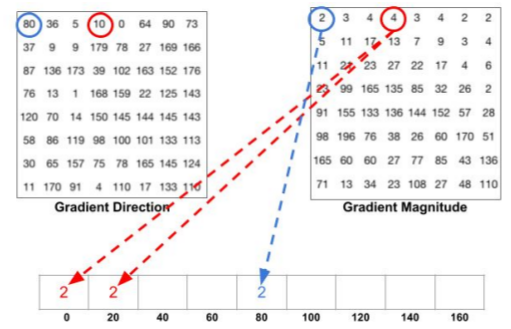
\includegraphics[width=0.5\textwidth]{./pictures/hogHist}
   	\caption{Cálculo histograma de gradientes}\label{fig: hogCalc}
\end{figure}
     La contribución de todos los pixeles in la celda de 8x8 son sumados para crear el histograma de 9 bins, para la celda de la figura \ref{fig: hog8x8} el histograma final se encuentra en la imagen \ref{fig: finalHist}, se puede notar que hay más en los bins cerca de los 0 y 180 grados, esto indica que los gradientes están apuntando arriba o abajo.
 \begin{figure}[htbp]
 	\centering
 	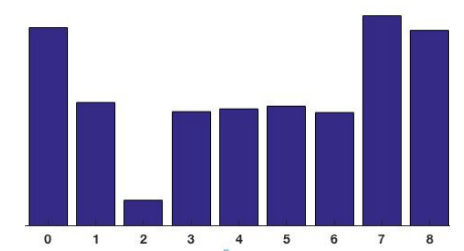
\includegraphics[width=0.5\textwidth]{./pictures/finalHist}
 	\caption{Histograma final de celda de 8x8}\label{fig: finalHist}
 \end{figure}    
     
 \subsubsection{Paso4: Normalización del bloque de 16x16}
 El histograma creado en las etapas anteriores está basado en los gradientes de la imagen, sin embargo, los gradientes en una imagen son sensibles a las variaciones de luz, para contrarrestar este problema en el artículo original de HOG [Dalal et al, 2005] el autor recomienda normalizar el histograma, él propone cuatro diferentes tipos de normalizaciones donde la más común es la normalización con la norma L2 o euclídea. Además, Dalal sugiere realizar la normalización en  bloques mayores del histograma correspondiente a la celda de 8x8 ya que de acuerdo a sus experimentos se obtienen resultados superiores.\\
 %So effective local contrast normalization turns out to be essential for good performance. We evaluated a number of different normalization schemes. Most of them are based on grouping cells into larger spatial blocks and contrast normalizing each block separately. The final descriptor  is then the vector of all components of the normalized cell  responses from all of the blocks in the detection window. This may seem redundant but good normalization is  critical and including overlap significantly improves the performance
 En el ejemplo del corredor y siguiendo las instrucciones de investigación original, se concatenan cuatro histogramas de 8x8 (histograma de 9x1) para formar un bloque de 16x16 y en consecuencia obtener un vector normalizado de 36x1. Luego, la ventana (bloque de 16x16) es desplazado cada 8 pixeles y de nuevo se calcula el vector normalizado. En la figura \ref{fig: hog16x16Block} se puede apreciar el proceso anterior del desplazamiento de la ventana
 \begin{figure}[htbp]
 	\centering
 	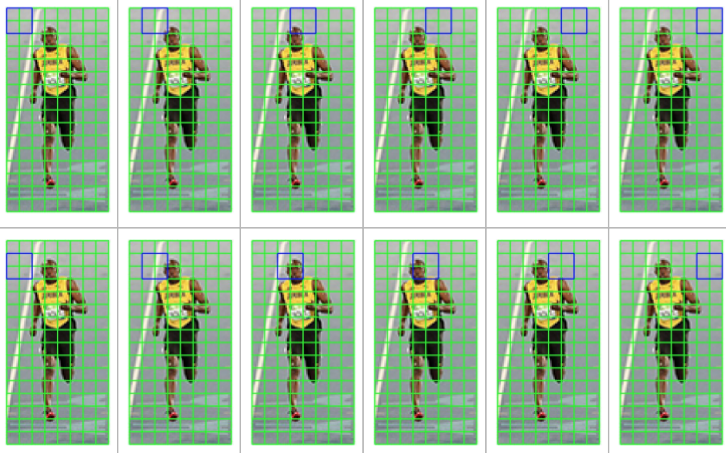
\includegraphics[width=0.6\textwidth]{./pictures/hog16x16Block}
 	\caption{Normalización enllevada a cabo desplazando los bloques de 16x16}\label{fig: hog16x16Block}
 \end{figure}      
     
  \subsubsection{Paso 5. Cálculo del vector de características HOG}
  El vector final de características para la región seleccionada se obtiene de la concatenación de los vectores de dimensión de 36x1,  tomando en consideración que hay 7 posiciones horizontales posibles de la región de la imagen, 15 verticales y cada bloque tiene un longitud de 36 elementos, el vector final tiene: 7*15*36=3780 elementos.\\
  Para la visualización unicamente se grafican los histogramas normalizados de 9x1 en las celdas de 8x8, imagen \ref{fig: hogVis}. Se puede percibir que las direcciones dominantes del histograma capturan la forma de la persona.
   \begin{figure}[htbp]
   	\centering
   	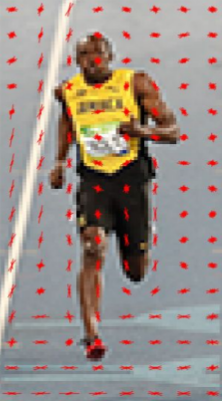
\includegraphics[width=0.3\textwidth]{./pictures/hogVis}
   	\caption{}\label{fig: hogVis}
   \end{figure}
     
     
     
     
     
     
     
     
     
     
     
     
     
     
     
     
     
     
     
     
     
     
     
     

